\documentclass{beamer}
\usepackage{graphicx, epstopdf}
\usepackage{grffile}
\usepackage{amsmath, amssymb, amsbsy, amstext}
% \usepackage{xcolor}

\usepackage[utf8]{inputenc}
\usepackage{natbib}

\usepackage{todonotes}
% \usepackage[disable]{todonotes}
\presetkeys{todonotes}{inline}{}

\usepackage{booktabs} % for much better looking tables
\usepackage{tabularx}

\newcommand{\code}[1]{{\texttt{#1}}}
\newcommand{\libraryname}[1]{{\texttt{#1}}}
\newcommand{\codefile}[1]{{\textit{#1}}}
\newcommand{\program}[1]{\code{#1}}
\newcommand{\taskname}[1]{{\textit{#1}}}
\newcommand{\newterm}[1]{{\textit{#1}}}
\newcommand{\scarequotes}[1]{`#1'}
\newcommand{\sampleswidth}{0.23\textwidth}
\newcommand{\samplesheight}{1.5cm}

% \definecolor{darkgreen}{rgb}{0,0.6,0}
% \usepackage{pgf}
% \logo{\pgfputat{\pgfxy(-2,6)}{\pgfbox[center,base]{\includegraphics[height=2cm]{amsilogo.jpg}}}}

\usetheme{Darmstadt}
%\usetheme{Dresden} %Dresden, Darmstadt, Warsaw
% \usecolortheme{dove}
% \title{Sphere Detection using Boosted Classifiers}
\title{A Study on Detecting Three-Dimensional Balls using Boosted Classifiers}
% \subtitle{Computer Vision Interim Report}
\author{Mitchell Metcalfe, Brendan Annable, Monica Olejniczak, Stephan K. Chalup}
\institute{The University of Newcastle, Australia}
\date{\today}

\begin{document}

	\maketitle


	% \begin{frame}{Object detection}
	% 	\begin{center}
	% 		To create an object detector using supervised learning, a correctly
	% 		labelled dataset needs to be created for training.
	% 	\end{center}
	% \end{frame}

\section{Introduction}

	\subsection{Motivation}

	\begin{frame}{Robot soccer}
		Robots at RoboCup \citep{KitanoAKNO97} need find the ball. A common approach is simple circle detection, which has problems: \par
		\begin{itemize}
			\item Centre circle
	        \item Penalty spots
	        \item Line intersections
	        \item Anything that looks round from some angle
		\end{itemize}
		\begin{center}
			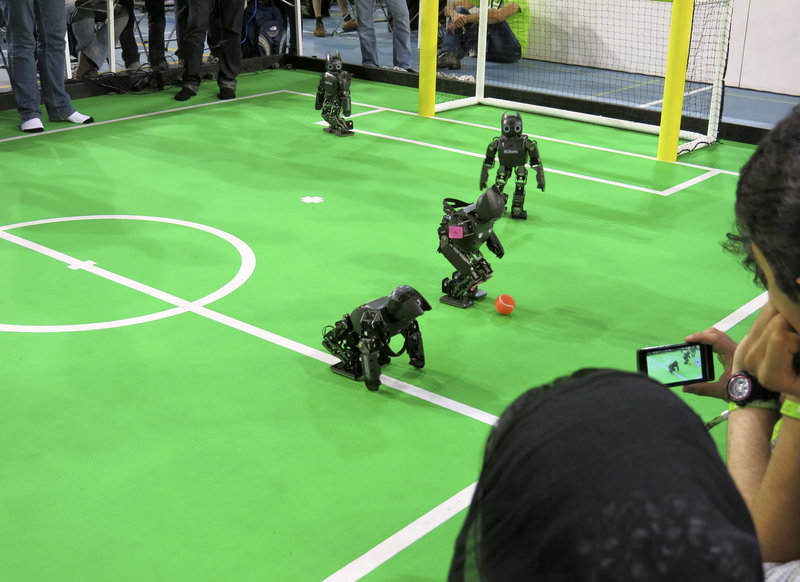
\includegraphics[height=4cm]{field2}
		\end{center}
	\end{frame}

	% \begin{frame}{Current approaches}
	% 	A review of recent literature reveals several recent approaches:
	% 	\todo{Something}
	% \end{frame}

	\begin{frame}{Sphere detection problem}
		\begin{itemize}
			\item More general problem than ball detction.
			\item Detect spheres.
			\item Do not detect any \scarequotes{round things} unless they are spheres.
		\end{itemize}
		\begin{table}[h]
			\centering
			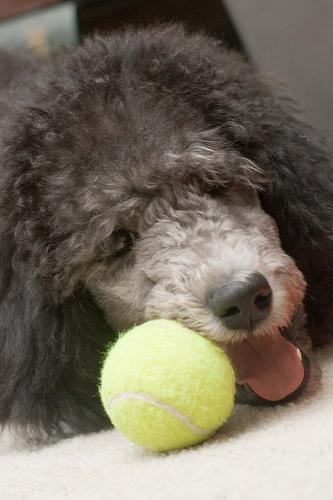
\includegraphics[height=4cm]{training_images/positive/n04409515_2793} \hspace*{0.1cm}
			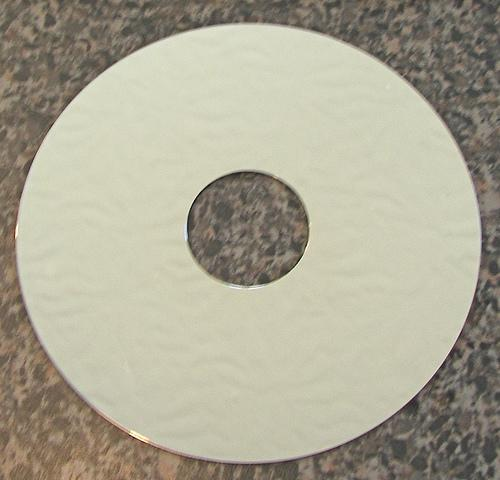
\includegraphics[height=4cm]{training_images/hard_negative/n03208556_9694}
		\end{table}
	\end{frame}

\section{Focus of work}
	\begin{frame}{Proposed approach}
		Attempt to solve the more generic problem of sphere detection using a boosted classifier cascade.
	\end{frame}

	\begin{frame}{Feature comparison}
		Compare appropriateness of the following feature types for the problem: \par
		\begin{itemize}
			\item Extended Haar features \citep{Lienhart2002extended}
			\item Local Binary Patterns (LBPs) \citep{liao2007learning}
			\item Histograms of Oriented Gradients (HoG) features \citep{dalal2005histograms}
		\end{itemize}
	\end{frame}

\section{Methodology}

\section{Training}

\begin{frame}{Dataset}
	All training and testing images were sourced from ImageNet \citep{imagenet_cvpr09}.
\end{frame}

\begin{frame}{Software used}
	\begin{itemize}
		\item Classifiers of each feature type were trained simultaneously
		\item Run on a Macbook Pro with an Intel Core i7 (I7-3740QM) processor and 16GB RAM.
	\end{itemize}
\end{frame}


\section{Results}

\begin{frame}{Feature performance comparison}
	Notable results: \par
	\begin{itemize}
		\item Haar features performed better than HOGS or LBP.
		\item LBP features performed better than HOGS.
		\item Increasing the proportion of negative images decreased the hit rate.
	\end{itemize}
\end{frame}

\begin{frame}{Future work}
	\begin{itemize}
		\item Image preprocessing techniques.
	\end{itemize}
\end{frame}

\subsection{Bibliography}

\begin{frame}{Bibliography}
	\footnotesize
	\bibliography{references}
	\bibliographystyle{apalike}
\end{frame}

\end{document}
